Write async
Async AGREE semantics and modelling (annotations, schedule, virtual events)

\begin{figure}[ht!]
\centering
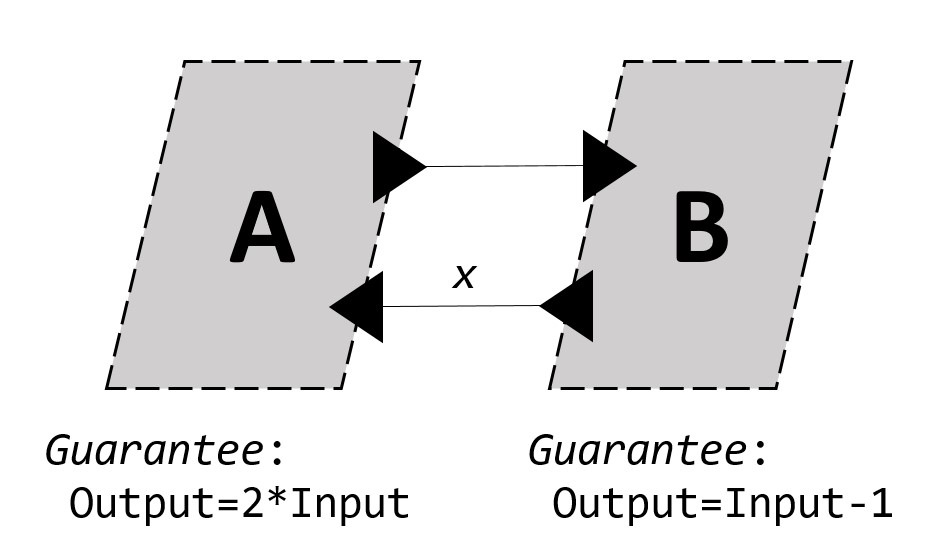
\includegraphics[width=60mm]{motivation.jpg}
\caption{An AADL Model with AGREE Contracts\label{motivation}}
\end{figure}

We use the AADL model annotated with AGREE contracts in Figure \ref{motivation} to illustrate the difference between the AGREE synchronous semantics and the AADL semantics. The model consists of two threads A and B. The AGREE contracts associated with each thread define the input output data relationship. Currently AGREE adopts a synchronous semantics. This means the communication between the two threads are instantaneous. And the two contracts have to be satisfied simultaneously. For example, the value of signal x is defined by the solution to the fix-point equation x = F(x), where F(x) = 2x -1. That is, \[x_0 = F(x_0), x_1 = F(x_1), x_2 = F(x_2), ...\]. This results in x = (1,1,1,…). However, in AADL a data port of a thread represents buffered communication.  In AADL reading is non-blocking. If a data buffer is empty, a pre-defined constant value or the previous value is used. Also the execution of the two threads could be in arbitrary order. Given a schedule (A,B,A,B,A,B,…) and an initial value x = 0,  by Kleene iteration: \[x_1 = F(x_0), x_2 = F(x_1), x_3 = F(x_2),...\] This results in x = (0,-1,-3,…). Clearly, the two traces are different. In other words, a property proved with synchronous AGREE semantics does not necessarily hold with AADL semantics.


